\section{Clustering}

The \textbf{classical clustering} problem starts with 

\begin{itemize}
    \item A set of $n$ objects;
    \item A $n \times n$ matrix $A$ of pairwise similarities that gives us an edge-weighted graph $G$.
\end{itemize}

, and the goal is to \textbf{partition} the vertices of $G$ into \textbf{maximally homogeneous groups (clusters)}. Usually we make the following assumptions:

\begin{itemize}
    \item The \textbf{similarity metric} is \textbf{symmetric}, i.e. $\text{sim}(a,b) = \text{sim}(b,a)$. However, this is not always the case: if, for example, we consider the case of computing a similarity between two documents represented using \textit{bag of words} (each document is represented as a probability distribution of its terms), then the \textit{KL divergence} can be used for computing the similarity, but we've seen that this measure is not symmetric;
    \item We only consider \textbf{pairwise similarities}, i.e. similarity between two objects. Notice that there are situations in which we may compute the similarity between more that 2 objects, e.g. with \textbf{tensors} or \textbf{hypergraphs}.
    \item The graph $G$ is an undirected graph.
\end{itemize}

\image{img/clustering}{The "classical" clustering problem.}{0.8}

Clustering problems abound in many areas of CS, e.g. image processing and CV, IR, document analysis, data mining etc.. If we consider, for example, the image segmentation problem, it's easy to see that it "simply" consists in clustering similar pixels of an image into coherent regions. 

\subsection{Feature-based clustering algorithm: K-means}
K-means is an iterative clustering algorithm that relies on the following assumptions:

\begin{itemize}
    \item It is provided as input with \textbf{feature vectors}, and for this reason we refer to K-means as a \textbf{feature-based} (or \textbf{central}) \textbf{clustering} algorithm, i.e. it receives in input points in a high-dimensional feature space. The other approach is represented by the \textbf{graph-based} (or \textbf{pairwise}) \textbf{clustering} algorithm, in which we are given either a \textbf{similarity matrix} or a \textbf{graph} in which the weights represent the similarity between the entities. In this latter case we do not make any assumption about the representations of the objects;
    \item The \textbf{number of clusters} is known in advance (in many applications this is a problem).
\end{itemize}

The algorithm follows these steps:
\begin{itemize}
	\item \textbf{Initialize:} pick $K$ random points as cluster centers.
	\image{img/kmeans1}{Initialization with $K=2$.}{0.24}
	\item \textbf{Alternate:}
	\begin{enumerate}
		\item \textbf{Assign} data points to \textbf{closest cluster center}.
		\item \textbf{Change the cluster center} to the \textbf{average} of its assigned points.
		\begin{figure}[H]
			\begin{minipage}[t]{0.42\linewidth} 
				\centering
				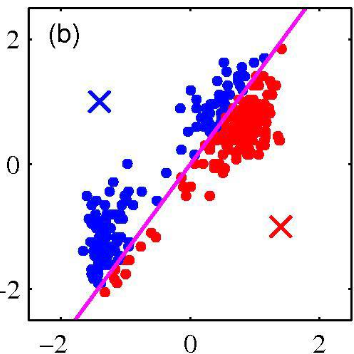
\includegraphics[width=0.58\textwidth]{img/kmeans2}
				\caption{Iterative step 1.}
			\end{minipage}        
			\hspace{2.5cm}
			\begin{minipage}[t]{0.42\linewidth} 
				\centering
				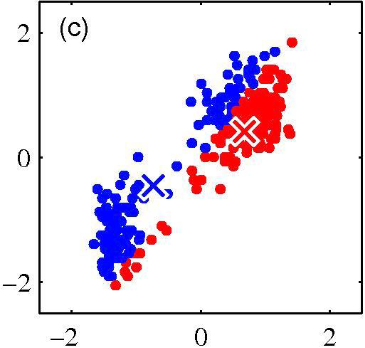
\includegraphics[width=0.58\textwidth]{img/kmeans3}
				\caption{Iterative step 2.}
			\end{minipage}
		\end{figure}
		\FloatBarrier
	\end{enumerate}
	\item \textbf{Stop:} when no points' assignments change.
	\begin{figure}[H]
		\begin{minipage}[t]{0.42\linewidth} 
			\centering
			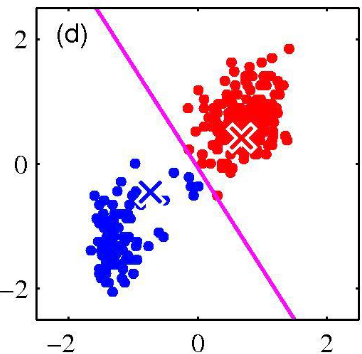
\includegraphics[width=0.58\textwidth]{img/kmeans4}
			\caption{Repeat until convergence.}
		\end{minipage}        
		\hspace{2.5cm}
		\begin{minipage}[t]{0.42\linewidth} 
			\centering
			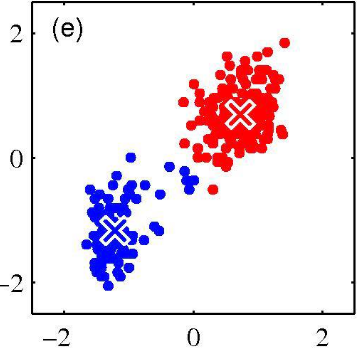
\includegraphics[width=0.58\textwidth]{img/kmeans5}
			\caption{Final output.}
		\end{minipage}
	\end{figure}
\end{itemize}
\paragraph*{Advantages of K-means.} 
\begin{itemize}
        \item It is a \textbf{simple algorithm};
	\item It is guaranteed to \textbf{converge} in a \textbf{finite number of steps};
	\item It \textbf{minimizes} an \textbf{objective function} (i.e. it \textbf{maximizes} the \textbf{compactness} of clusters):
	$$\sum_{i \in \text{clusters}} \Biggl\{ \sum_{j \in \text{elements of i-th cluster}} ||x_j - \mu_i||^2 \Biggr\}$$
	where $\mu_i$ is the center of cluster $i$;
	\item It \textbf{assigns} data points to closest cluster center in $O(Kn)$ and it \textbf{changes} the cluster center to the average of its points in $O(n)$, so it is an \textbf{efficient} algorithm.
\end{itemize}

\paragraph{Disadvantages of K-means}

\begin{itemize}
    \item It converges to a \textbf{local minimum} of the error function, i.e. we have no theoretical guarantees that the algorithm will converge to a global minimum, and that's the reason why we may run the algorithm several times;
    \item It needs to pick $K$ \textbf{initial points}, hence proving to be very \textbf{sensitive to the initialization step};
    \item It is also very sensitive to the \textbf{outliers}, which are not known in advance;
    \item It only finds \textbf{spherical clusters}, due to the objective function it minimizes. In this sense, this algorithm does not work when we have non-convex clusters;
    \item It works with \textbf{feature vectors}, which sometimes are not easy to obtain.
\end{itemize}

\subsection{Eigenvector-based clustering}
As we introduced before, the other possible approach for unsupervised learning is represented by the \textbf{graph-based clustering}, in which the input is represented either by a \textbf{similarity matrix} or a \textbf{graph}.

\begin{figure}[h!]
		\centering
		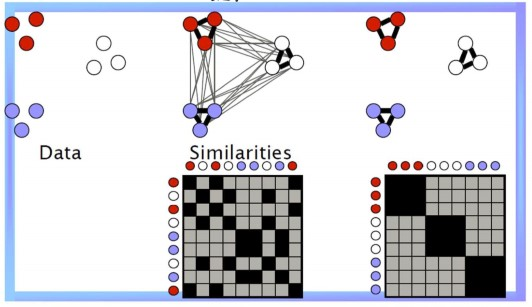
\includegraphics[scale = 1.5]{img/graph matrix clustering.jpg}
		\label{svm}
		\caption{Graph and matrices for clustering}
\end{figure}

It is important to underline the fact that the two representations are equivalent, but they have different characteristics:

\begin{itemize}
    \item If we consider the \textbf{similarity matrix}, then eivenvalues and eigenvectors play a crucial role in the clustering problem, since they provide an information of the matrix which is independent of the permutations of the matrix. In this sense, despite the fact that there may exist many matrices representing the same graph, the resulting eigenpairs remain the same;
    \item If we consider the \textbf{graph} representation, then the notion of \textbf{cut} plays a crucial role in clustering: this problem, indeed, reduces in finding the cut(s) of the graph which separate the object of different classes from the others, i.e. that maximize the \textbf{intra-class similarity} and minimize the \textbf{inter-class similarity}. 
\end{itemize}

We now focus on the clustering problem that deals with a \textbf{similarity matrix}.
\subsubsection{Eigenvalues and eigenvectors}
Before defining the clustering problem as a \textbf{eigenvector-based} problem, we make a little digression on eigenpairs. We first focus on two cases:

\begin{itemize}
    \item Suppose we have a \textbf{symmetric matrix} $A$, then all the \textbf{eigenvalues} are \textbf{real}, which means we can consider an order between the eigenvalues. This property introduces a very strong assumption of the \textbf{spectral graph theory}, i.e. that the input matrix must be symmetric;
    \item Suppose we have a \textbf{non symmetric matrix} $A$, then $A$ must be symmetrized, i.e. we must build a symmetrix matrix $A'$ as:

    $$
    A' = \frac{1}{2} (A + A^T)
    $$
\end{itemize}

Now, suppose that the matrix $A$ is symmetric, we can compute the largest eigenvalue $\lambda_\text{MAX}$ of $A$ by solving one of the following two maximization problem:

\begin{equation}\label{eq_largest lambda1}
\lambda_\text{MAX} = \max_{x} \quad & x^T A x\\
\quad \textrm{ s.t.} \quad & x^T x = 1
\end{equation}

or

\begin{equation}\label{eq_largest lambda2}
\lambda_\text{MAX} = \max_{x} \quad & \frac{x^T A x}{x^T x}\\
\quad \textrm{ s.t.} \quad & x \in \mathbb{R}^n
\end{equation}

, where $\frac{x^T A x}{x^T x}$ is defined as \textbf{Rayleigh quotient}. Notice that \ref{eq_largest lambda1} is a \textbf{constrained optimization problem}, while \ref{eq_largest lambda2} is an \textbf{unconstrained optimization problem}.

On the other hand, the general eigenvector/eigenvalue problem is defined by finding the $\lambda$ s.t. $Ax = \lambda I x$, where $I$ represents the \textbf{identity matrix}: if we have another matrix $B$, then the solution becomes $Ax = \lambda B x$, and the solution of finding $\lambda_\text{MAX}$ is:

\begin{equation}\label{eq_largest lambda3}
\max_{\lambda_\text{MAX}} \quad & \frac{x^T A x}{x^T B x}\\
\quad \textrm{ s.t.} \quad & x \in \mathbb{R}^n
\end{equation}

\subsubsection{Problem definition}
Let us represent a \textbf{cluster} using a \textbf{vector} $x$ whose $i$-th entry captures the participation of node $i$ in that cluster:

$$x_i : \begin{cases}
\neq 0 \text{  if } i \in C\\
= 0 \text{  if } i \notin C
\end{cases}$$

If a node does not participate in a cluster, the corresponding entry is zero. We also impose the \textbf{restriction} that $x^Tx = 1$ in order to avoid the trivial solution $x=0$.\\
Thus, we want to maximize:
$$\sum_{i=1}^n \sum_{j=1}^n w_{ij} x_i x_j = x^TAx$$
which measures the \textbf{cluster's cohesiveness}. In this sense, out goal is to maximize the internal similarity of the points within the cluster. As we introduced in the previous section, this is an \textbf{eigenvalue problem}, which consists in choosing the \textbf{eigenvector} of $A$ corresponding to the \textbf{largest eigenvalue}.\\

From the following image we can see that it could be possible to find clusters by visual inspection of the eigenvectors.

\begin{figure}[H]
	\begin{minipage}[t]{0.49\linewidth} 
		\centering
		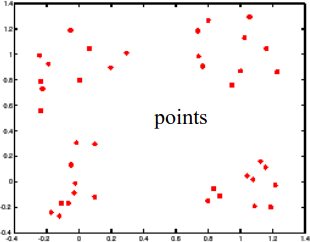
\includegraphics[width=1\textwidth]{img/eigenpoints}
	\end{minipage}        
	\hspace{1cm}
	\begin{minipage}[t]{0.49\linewidth} 
		\centering
		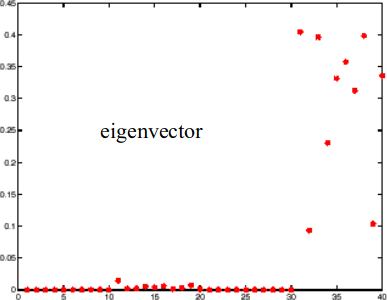
\includegraphics[width=1\textwidth]{img/eigenvectors}
	\end{minipage}
\end{figure}

However, solving the previous problem only allows to find a \textbf{single cluster}, so in case we must extract \textbf{more than two clusters} from the eigenvectors, we can consider one of the following strategies:

\begin{enumerate}
    \item Recursively split each side to get a tree, continuing till the eigenvalues are too small;
    \item Use not only the largest eigenvalue, but also the others. A powerful result in linear algebra says that the second largest eigenvalue (i.e. the eigenvalue associated to the second largest eigenvector) can be obtained by considering 

    \begin{equation}\label{eq_largest lambda3}
    \max \quad & \frac{x^T A x}{x^T x}\\
    \quad \textrm{ s.t.} \quad & x \in \mathbb{R}^n \text{and } x \perp x_\text{max}
    \end{equation}
    , where $x_\text{max}$ represents the eigenvector associated to the largest eigenvalue.
    
\end{enumerate}

\subsubsection{Clustering by eigenvectors : algorithm}
The algorithm that builds the clusters through the eigenvectors performs the following steps:
\begin{enumerate}
	\item Construct (or take as input) the \textbf{affinity matrix} $A$;
	\item Compute the \textbf{eigenvalues} and \textbf{eigenvectors} of $A$;
	\item Repeat until there are sufficient clusters:
	\item $\quad$ Take the \textbf{eigenvector} corresponding to the \textbf{largest} unprocessed \textbf{eigenvalue};
	\item $\quad$ \textbf{Zero} all the components corresponding to \textbf{elements} that have already \textbf{been clustered};
	\item $\quad$ \textbf{Threshold} the remaining components to determine which elements belong to this cluster;
	\item $\quad$ If all elements have been accounted for, there are sufficient clusters;
\end{enumerate}

\subsection{Graph-based clustering algorithm}
If we consider the \textbf{graph} representation we have that:
\begin{itemize}
	\item A \textbf{node} represents each of the \textbf{pixels};
	\item An \textbf{edge} between every pair of pixels (or every pair of "sufficiently close" pixels), which is weighted according to the affinity or \textbf{similarity} of the two nodes.
\end{itemize}  
\image{img/imageasgraph}{Image as a graph.}{0.7}
If we suppose to represent each \textbf{pixel} with a \textbf{feature vector} $x$ and to define a \textbf{distance function} appropriate for this feature representation, then we can \textbf{convert} the \textbf{distance} between two feature vectors into an \textbf{affinity} with the help of a \textbf{Gaussian kernel}:
$$exp\left(-\frac{1}{2\sigma^2} dist(x_i, x_j)^2\right)$$
Notice that we can exploit this kernel to transform a feature-based dataset into a graph-based one. We can notice that the \textbf{similarity} of two data points is \textbf{inversely proportional} to their \textbf{distance}, and we also underline the importance of the \textbf{scale} parameter $\sigma$: the \textbf{smaller} $\sigma$, the \textbf{more rigid} will be the clustering algorithm in grouping together only nearby points; on the other hand, the \textbf{larger} $\sigma$, the more the algorithm will \textbf{group} together \textbf{far-away points}.

We now focus on the clustering as a \textbf{graph partitioning problem}. Let $G=(V,E,w)$ be an undirected weighted graph, i.e. the similarity matrix is symmetric, and given a partition (or cut) $(C_1, C_2)$ of the graph $G$, then the following quantity can be defined:

$$
cut(C_1,C_2) = \sum_{i \in C_1} \sum_{j \in C_2} w(i,j)
$$

In Picture \ref{cut}, the cut of the two sub graphs is given by the sum of the weights of the red edges.

\begin{figure}[h!]
		\centering
		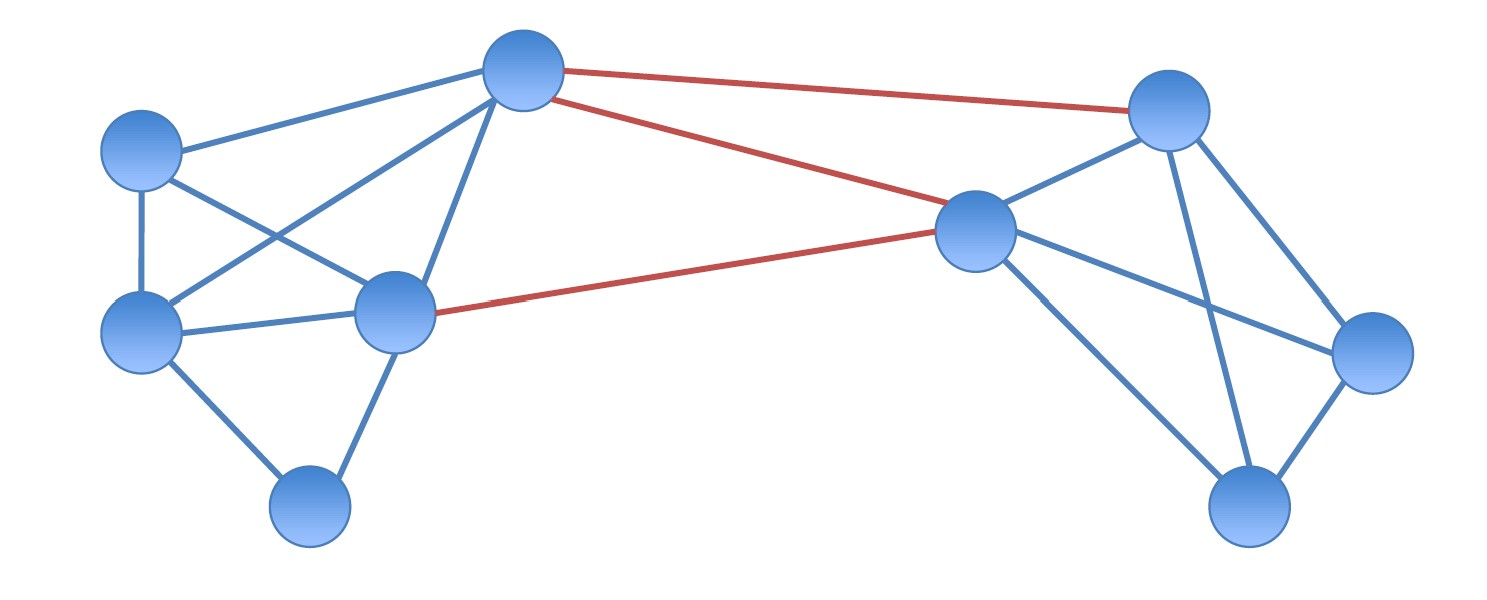
\includegraphics[scale = 0.6]{img/cut.jpg}
		\label{cut}
		\caption{Cut in a graph}
\end{figure}

\paragraph{Minimum cut}
\\
Given this quantity, we can easily connect the problem of determine the clusters of a graph to the one of finding a cut that maximizes the intra-cluster similarity and minimizes the inter-class similarity of the points contained in the two partitions that are formed. More specifically, finding the clusters in a graph is equal to solve the so called \textbf{minimum cut problem}. This problem tries to find the cut that minimizes the quantity $cut(C_1, C_2)$ among all the possible cuts, i.e. partitions, $(C_1, C_2)$.

Despite the fact that the number of cuts in a graph grows exponentially with the number of nodes, an important property of the \textit{minimum cut} problem is that it is solvable in polynomial time. However, a quite important disadvantage of this problem is that it favors highly unbalanced clusters, in particular the ones composed by single vertices, as represented in Picture \ref{problem}.

\begin{figure}[h!]
		\centering
		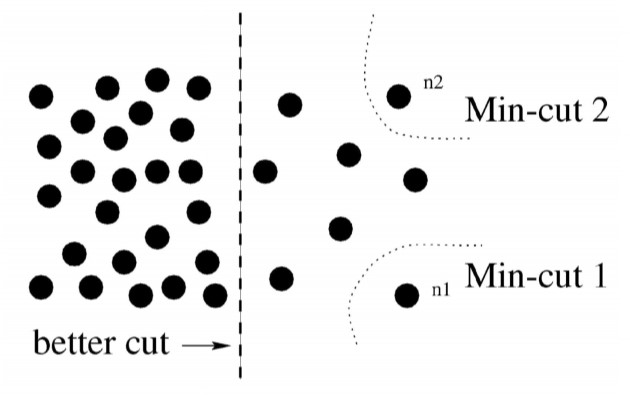
\includegraphics[scale = 1.0]{img/min cut problem.jpg}
		\label{problem}
		\caption{Disadvantage of MinCut problem: isolated vertices form a cluster}
\end{figure}

This problem derives from the fact that it takes into account only the intra-cluster similarity, resulting in this kind of undesired partitions.

\paragraph{Normalized cut}
\\
The other possible approach when dealing with graph partitioning, and the one adopted in this project, is represented by solving the \textbf{normalized cut} problem. Before discussing the details of this problem, we introduce some important metrics:

\begin{itemize}
    \item the \textit{degree} of a node is defined as $\text{deg}(i) = \sum_j w_{i,j}$, i.e. it is represented by the sum of the values in the i-th row of the matrix representing the graph;
    \item the \textit{volume} of a set of nodes is defined as $vol(A) = \sum_{i \in A} d_i$, where $A \subseteq V$, i.e. it is represented by the sum of the degrees of the nodes in the set (sum of multiple rows).
\end{itemize}

The idea of \textit{normalized cut} is to overcome the limits of \textit{minimum cut} by normalizing the previous quantity by a measure (the volume) that allows to combine both the intra-cluster similarity and the inter-cluster similarity. More specifically, for the \textit{normalized cut} problem, the quantity that has to be minimized is the following one:

$$
Ncut(C_1,C_2) = cut(C_1, C_2) \left( \frac{1}{vol(C_1)} + \frac{1}{vol(C_2)} \right)
$$

Despite providing more accurate clusters, the crucial issue about \textit{normalized cut} is that finding its minimum is \textbf{NP-hard}, and for this reason there exist some efficient approximations that exploit the properties of linear algebra. One of this approximations is based on the \textbf{graph Laplacian} or \textbf{Laplacian matrix}, which is a matrix defined as:

$$
L = D - W
$$

, where:

\begin{itemize}
    \item $D$ is the \textit{diagonal degree matrix}, i.e. $d_{ii} = \text{deg}(i) = \sum_j w_{i,j}$;
    \item $W$ is the \textit{similarity matrix}, in which the elements of the diagonal are equal to 0 by definition. Moreover, if the graph is unweighted, then $W$ only contains 1s and 0s. 
\end{itemize}

In this sense, the elements of $L$ are given by:

$$
L _ { i , j } = \left\{ \begin{array} { l l } { \operatorname { d } \left( v _ { i } \right) } & { \text { if } i = j } \\ 
{ - 1 } & { \text { if } i \neq j \text { and } v _ { i } \text { is adjacent to } v _ { j } } \\ 
{ 0 } & { \text { otherwise } } \end{array} \right.
$$

This is an example of the degree matrix $D$ and the affinity matrix $W$ in relation to the graph of the next page.
\begin{figure}[H]
	\begin{minipage}[t]{0.49\linewidth} 
		\centering
		$$ D = \begin{bmatrix}
		2 & 0 & 0 & 0 & 0 & 0 \\
		0 & 4 & 0 & 0 & 0 & 0 \\
		0 & 0 & 4 & 0 & 0 & 0 \\
		0 & 0 & 0 & 1 & 0 & 0 \\
		0 & 0 & 0 & 0 & 3 & 0 \\
		0 & 0 & 0 & 0 & 0 & 2 \\
		\end{bmatrix}$$
		\caption{Degree matrix $D$.}
	\end{minipage}        
	\hspace{1cm}
	\begin{minipage}[t]{0.49\linewidth} 
		\centering
		$$ W = \begin{bmatrix}
		0 & 1 & 1 & 0 & 0 & 0 \\
		1 & 0 & 1 & 1 & 1 & 0 \\
		1 & 1 & 0 & 0 & 1 & 1 \\
		0 & 1 & 0 & 0 & 0 & 0 \\
		0 & 1 & 1 & 0 & 0 & 1 \\
		0 & 0 & 1 & 0 & 1 & 0 \\
		\end{bmatrix}$$
		\caption{Affinity matrix $W$.}
	\end{minipage}
\end{figure}

\image{img/graphLaplacian}{Example of laplacian graph.}{0.85}

The \textit{Laplacian matrix} $L$ satisfies the following \textbf{properties}:
\begin{enumerate}
        \item $L \in \mathbb{R}^{n \times n}$ and the sum of rows/columns is always 0;
	\item For all vectors $x$ in $\mathbb{R}^n$, we have:
	$$x ^ T L x = \frac { 1 } { 2 } \sum _ { i, j = 1 } ^ { n } w _ { i j } \left( x _ { i } - x _ { j } \right) ^ { 2 } \geq 0$$
	This is proved as follows:
	$$\begin{aligned} 
	x ^ { T } L x & = x^T (D-W) x = x ^ { T } D x - x ^ { T } W x = \sum _ { i=1 }^n d _ { i } x _ { i } ^ { 2 } - \sum _ { i , j =1 }^n x _ { i } x _ { j } w _ { i j } \\ 
	& = \frac{1}{2} \left( \sum_i \sum_j d_{ij} x_i x_j - 2 \sum_i \sum_j w_{ij} x_i x_j + \sum_i \sum_j d_{ij} x_i x_j \right) \\ 
        & = \frac{1}{2} \left( \sum_i d_{ii} x_i^2 - 2 \sum_i \sum_j w_{ij} x_i x_j + \sum_j d_{jj} x_j^2 \right) \\
        & = \frac{1}{2} \left( \sum_i (\sum_j) w_{ij} \right) x_i^2 - 2 \sum_i \sum_j w_{ij} x_i x_j + \sum_j (\sum_i w_{ji}) x_j^2 \\
        & = \frac{1}{2} \left( \sum_i \sum_j w_{ij}x_i^2 - 2 \sum_i \sum_j w_{ij}x_i x_j + \sum_i \sum_j w_{ij} x_j^2 \right) \\
        & = \frac{1}{2} \left( \sum_i \sum_j w_{ij} (x_i^2 - 2 x_i x_j + x_j^2) \right) \\
        & = \frac{1}{2} \left( \sum_i \sum_j w_{ij} (x_i - x_j)^2 \right)

	\end{aligned}$$

        However, since both $w_{ij}$ and $(x_i - x_j)^2$ are $\geq 0$, then $x^TLx \geq 0$.
	 
	\item $L$ is a \textbf{symmetric} and \textbf{positive semi-definite} matrix. The symmetry of $L$ follows directly from the symmetry of $W$ and $D$, while the positive semi-definiteness is a direct consequence of the first property, which shows that $x ^ { T } L x \geq 0$. Notice that the positive semi-definiteness implies that all the eigenvalues are non negative, which has crucial consequences in optimization;
	 
	\item The smallest eigenvalue of $L$ is 0 and the corresponding eigenvector is the constant 1 vector. Moreover, $L$ has $n$ non-negative, real-valued eigenvalues $0 = \lambda _ { 1 } \leq \lambda _ { 2 } \leq \ldots \leq \lambda _ { n }$.
 
\end{enumerate}

More specifically, an important consequence of these properties is that the \textbf{multiplicity}, i.e. the number of eigenvectors associated to a specific eigenvalue, of the smallest eigenvalue $\lambda_1=0$ is the \textbf{number of connected components} $A_1, \dots, A_k$ of the graph. 

\paragraph{The normalized graph Laplacians} There are two matrices which are called normalized graph Laplacians in the literature. Both matrices are closely related to each other and are defined as:
$$\begin{array} { l } { L _ { \mathrm { sym } } = D ^ { - 1 / 2 } L D ^ { - 1 / 2 } = I - D ^ { - 1 / 2 } W D ^ { - 1 / 2 } } \\ { L _ { \mathrm { rw } } = D ^ { - 1 } L = I - D ^ { - 1 } W } \end{array}$$
We denote the first matrix by $L_{sym}$ as it is a symmetric matrix, and the second one by $L_{rw}$ as it is closely connected to a random walk.

\subsubsection{Solving normalized cut}
Any cut $(A,B)$ can be represented by a binary indicator vector $x$:

$$
x_i = \begin{cases}
+1 \text{  if } i \in A\\
-1 \text{  if } i \in B
\end{cases}
$$

, and it can be shown that:

$$
\min_x ~ \text{Ncut}(x) = \min_y \underbrace{\frac{y^T(D-W)y}{y^TDy}}_{\text{Rayleigh quotient}}
$$

subject to the constraint that $y ^ { \prime } D = \sum_{i} y_{i} d _ { i } = 0$, with $y _ { i } \in \{ 1 , - b \}$. Indeed, $y$ is an indicator vector with 1 in the $i$-th position if the $i$-th feature point belongs to $A$, negative constant ($-b$) otherwise ). Again, this problem is still \textbf{NP-hard}, so if we \textbf{relax} the constraint of $y$ to be a discrete-valued vector and allow it to take on real values, the original problem
$$
\min _ { y } \frac { y ^ T ( D - W ) y } { y ^ T D y }
$$

will be equivalent to:
$$
\min _ { y }  y ^ T ( D - W ) y \quad \text { s.t. } \quad y ^ T D y = 1
$$

This amounts to solve a \textit{generalized} eigenvalue problem:
$$
\underbrace{(D-W)}_{Laplacian}y=\lambda D y
$$

\paragraph{2-ways Ncut} Finally, we can provide a \textbf{solution} of the \textit{normalized cut} problem by exploiting this \textbf{algorithm}:

\begin{enumerate}
	\item Represent the \textbf{data points} as a \textbf{weighted graph} $G = (V,E)$, compute the weights of each edge and summarize them into $D$ and $W$;
	\item Solve the generalized eigenvalue problem $(D-W)y = \lambda Dy$ for the \textbf{eigenvector} associated the \textbf{second smallest eigenvalue} (we choose the second smallest eigenvalue since the eigenvector associated to the smallest eigenvalue is equal to 1, while the smallest eigenvalue is equal to 0, and it corresponds to the trivial partition $A = V$ and $B = \{\}$);
	\item Use the entries of the eigenvector to create a partition of the graph into two parts.
\end{enumerate}

Sometimes there's not a \textbf{clear threshold} to split based on the second vector since it takes continuous values. In which way it is possible to choose the splitting point?
\begin{itemize}
	\item Pick a constant value (0 or 0.5).
	\item Pick the median value as splitting point.
	\item Look for the splitting point that has minimum Ncut value:
	\begin{enumerate}
		\item Choose $n$ possible splitting points.
		\item Compute Ncut value.
		\item Pick minimum.
	\end{enumerate}
\end{itemize}

\subsubsection{Relaxation}
As we can see, in order to formalize the \textit{minimum cut problem} we had to \textbf{relax} the constraint owf $y$: the goal of relaxation is then to \textbf{relax the constraints} of a difficult problem and to solve the simpler problem. If we're lucky, the solution we obtain satisfies the original constraints, so we found a solution of the original problem, otherwise we can choose the nearest point that satisfies the original constraints.

Through relaxation we lose some precision in the final solution. Note that the \textbf{original} normalized cut problem returns \textbf{binary values} $(-1,1)$, indicating clustering membership. The \textbf{relaxed version}, on the right, returns \textbf{continuous values}. It may happen that \textbf{some points do not clearly belong to a specific cluster}, as they are close to the margin between the two clusters. For this reason the relaxed solution is \textbf{not} always in a \textbf{one-to-one correspondence} with the original problem, and choosing a ``\textbf{correct}'' threshold is very important.
\imageb{img/relaxation1}{0.8}

\subsubsection{Normalized cut with more than 2 clusters}
There are two possible approaches if we desire to obtain more than 2 clusters:
\paragraph*{Approach \#1.} It recursively performs the 2-way Ncut algorithm until we obtain the desired number of clusters (not so common).
\begin{enumerate}
	\item Given a weighted graph $G=(V,E,w)$, summarize the information into matrices $W$ and $D$.
	\item Solve $(D-W)y = \lambda Dy$ for eigenvectors with the smallest eigenvalues.
	\item Use the eigenvector with the second smallest eigenvalue to bipartition the graph by finding the splitting point such that Ncut is minimized.
	\item Decide if the current partition should be subdivided by checking the stability of the cut, and make sure Ncut is below the prespecified value.
	\item Recursively repartition the segmented parts if necessary.
\end{enumerate}
\textbf{Note:} this approach is \textbf{computationally wasteful}, only the second eigenvector is used, whereas the next few small eigenvectors also contain useful partitioning information.

\paragraph*{Approach \#2.} Using the first $k$ eigenvectors (far more popular).
\begin{enumerate}
	\item Construct a similarity graph and compute the unnormalized graph Laplacian $L$.
	\item Compute the $k$ smallest \textbf{generalized} eigenvectors $u _ { 1 } , u _ { 2 } , \dots , u _ { k }$ of the generalized eigenproblem $L u = \lambda D u$.
	\item Let $U = \left[ u_1, u_{ 2 }, \dots, u_{ k } \right] \in \mathbb { R } ^ { n \times k }$, i.e. the columns are the $k$ eigenvectors we computed.
	\item Let $y_i \in \mathbb{ R }^k$ be the vector corresponding to the $i$th row of $U$.
	$$U = \left[ \begin{array} { c c c c } { u _ { 11 } } & { u _ { 12 } } & { \cdots } & { u _ { 1 k } } \\ { u _ { 21 } } & { u _ { 22 } } & { \cdots } & { u _ { 2 k } } \\ { \vdots } & { \vdots } & { \ddots } & { \vdots } \\ { u _ { n 1 } } & { u _ { n 2 } } & { \cdots } & { u _ { n k } } \end{array} \right] = \left[ \begin{array} { c } { y _ { 1 } ^ { T } } \\ { y _ { 2 } ^ { T } } \\ { \vdots } \\ { y _ { n } ^ { T } } \end{array} \right]$$
	\item Thinking of $y_i$'s as points in $\mathbb{ R }^k$, cluster them with $k$-means algorithms. Why do we use k-means? The rows of $U$ allow to map the vertices of the graph in a 2-dimensional vector (like a projection), and it was proved that this mapping facilitates the use of the k-means algorithm.
\end{enumerate}

\textbf{Note:} the number $k$ of clusters must be known in advance.

\subsubsection{Spectral clustering vs $k$-means}
First of all, let us define the intuition behind \textbf{spectral clustering}: its goal is to cluster data that is connected but not necessarily compact or clustered within convex boundaries. This algorithm is very similar to the previous one, but it has 2 main differences; it works as follows
\begin{enumerate}
	\item Construct a similarity graph and compute the normalized graph Laplacian $L_{sym}$.
	\item Embed data points in a low-dimensional space (spectral embedding), in which the clusters are more obvious, computing the $k$ smallest eigenvectors $v_1, \dots, v_k$ of $L_{sym}$. 
	\item Let $V=\left[v_1,\dots, v_k \right] \in \mathbb{ R }^{n \times k}$.
	\item Form the matrix $U \in \mathbb{ R }^{n \times k}$ from $V$ by normalizing the row sums to have norm 1, that is: 
	$$u_ { i j } = \frac { v _ { i j } } { \left( \sum _ { k } v _ { i k } ^ { 2 } \right) ^ { 1 / 2 } }$$
	\item For $i=1,\dots, n$, let $y _ { i } \in \mathbb { R } ^ { k }$ be the vector corresponding to the $i$th row of $U$.
	\item Cluster the points $y_i$ with $i=1,\dots,n$ with the $k$-means algorithm into clusters $C_1, \dots, C_k$.
\end{enumerate}
The differences with the previous algorithm are following:

\begin{itemize}
    \item We compute a \textbf{normalized graph Laplacian} $L_{\text{sym}}$;
    \item The rows of $U$ are normalized to norm 1.
\end{itemize}

Applying $k$-means to Laplacian eigenvectors allows us to find \textbf{cluster} with \textbf{non-convex boundaries}.

\imageb{img/spectral1}{0.65}
\imageb{img/spectral2}{0.65}
\imageb{img/spectral3}{0.65}

As we said before, one of the main \textbf{issue} of k-means is represented by the choice of the value of $k$: one of the possible solutions (called \textbf{eigengap heuristic}) is to choose $k$ such that all eigenvalues $\lambda_1, \dots, \lambda_k$ are very small, but $\lambda_{k+1}$ is relatively large. In this way, the choosing of $k$ maximizes the eigengap (difference between consecutive eigenvalues) $\delta_k = |\lambda_k - \lambda_{k-1}|$.
\imageb{img/eigengap}{0.75}
